\documentclass{article}

\usepackage{amsfonts}
\usepackage{graphicx}
\usepackage{amssymb}
\usepackage{amsmath}
\usepackage{listings}


\DeclareMathOperator{\sech}{sech}
\newcommand{\NN}{\mathbb{N}}
\newcommand{\RR}{\mathbb{R}}
\newcommand{\QQ}{\mathbb{Q}}
\newcommand{\ZZ}{\mathbb{Z}}
\newcommand{\dV}{\;\mathrm{d}V}
\newcommand{\dA}{\;\mathrm{d}A}
\newcommand{\dx}{\;\mathrm{d}x}
\newcommand{\dy}{\;\mathrm{d}y}
\newcommand{\dz}{\;\mathrm{d}z}
\newcommand{\cA}{\mathcal{A}}
\newcommand{\Bb}{\mathcal{B}}
\newcommand{\Ww}{\mathcal{W}}
\newcommand{\Dd}{\mathcal{D}}
\newcommand{\Ss}{\mathcal{S}}
\newcommand{\Ee}{\mathcal{E}}
\DeclareMathOperator{\im}{im}


\setlength\parindent{18pt}

\begin{document}

Section 5.3:

8) The eigenvalues and eigenvectors of the coefficient matrix are complex.
Since it has complex eigenvalues, it is either a center or spiral.
Since the real part is essentially zero, that means the phase diagram is a center.

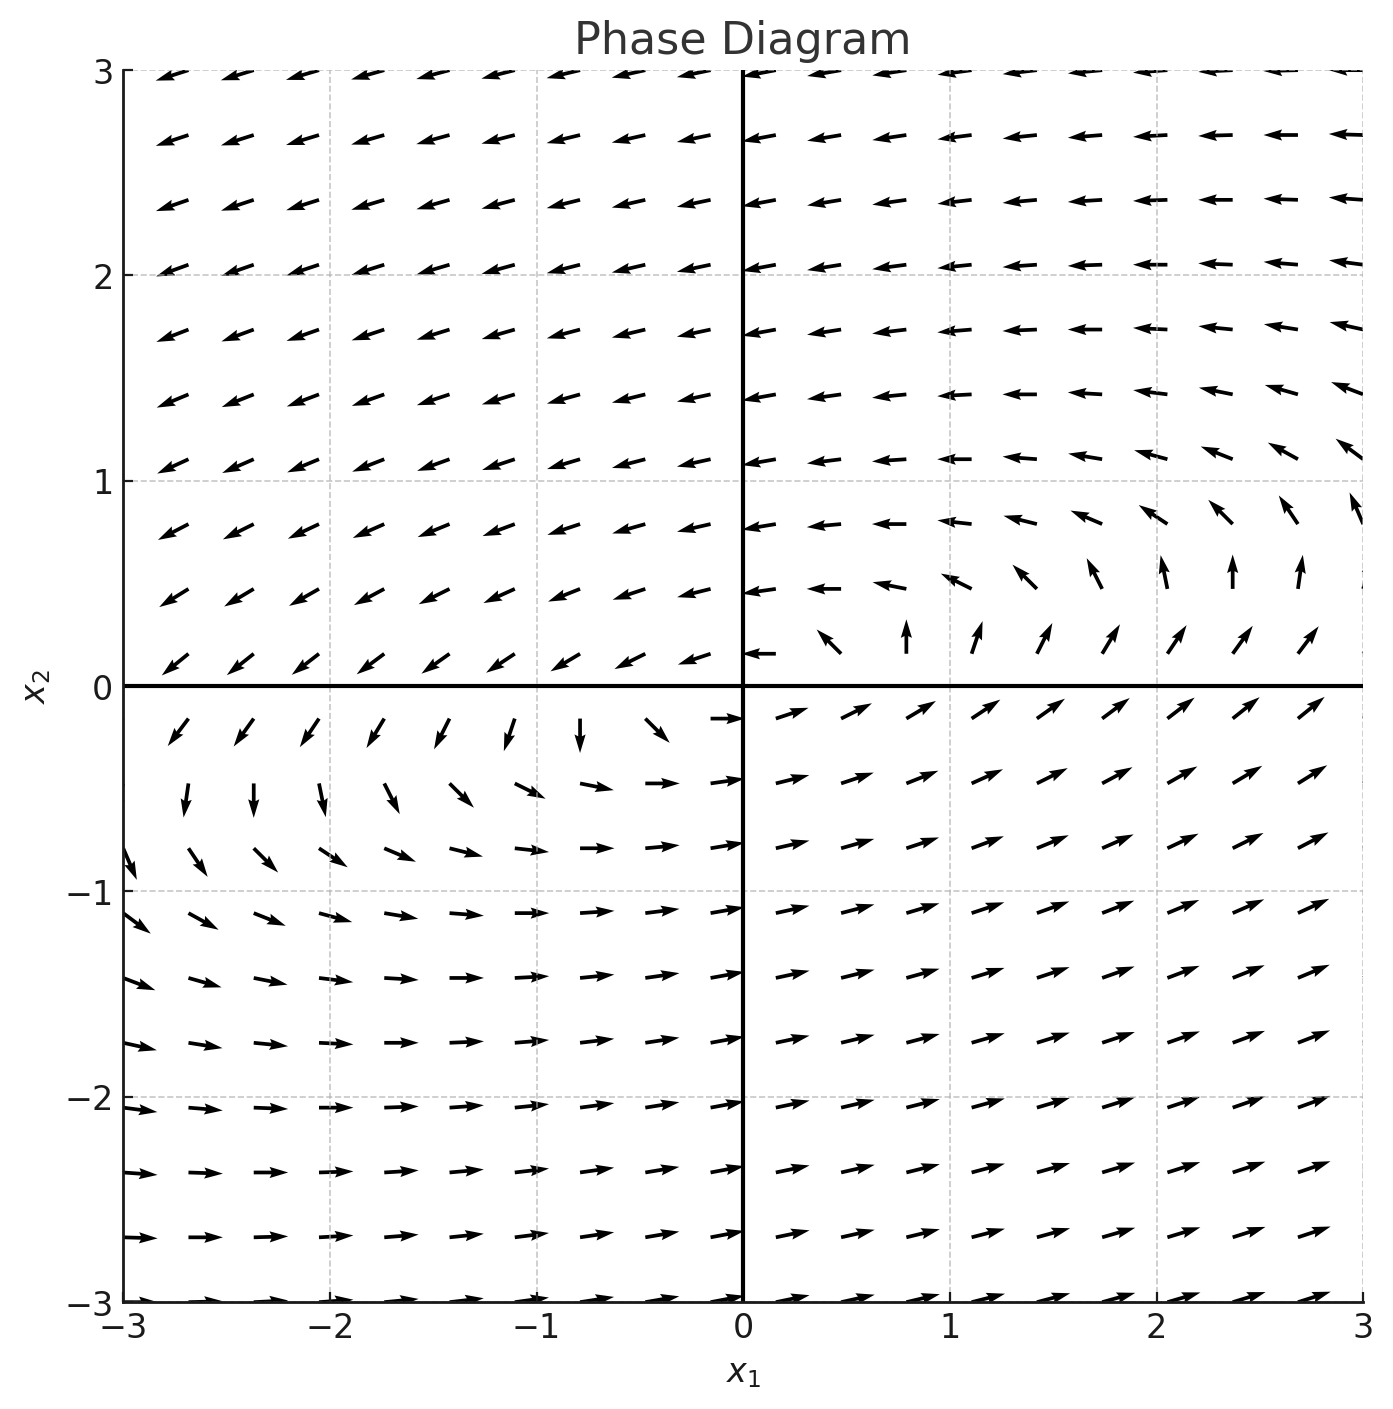
\includegraphics[width=\linewidth]{5_3_8_phase_diagram}


16) The eigenvalues are -10 and -100. The corresponding eigenvectors
are both real and distinct. Therefore, it forms an improper nodal sink.

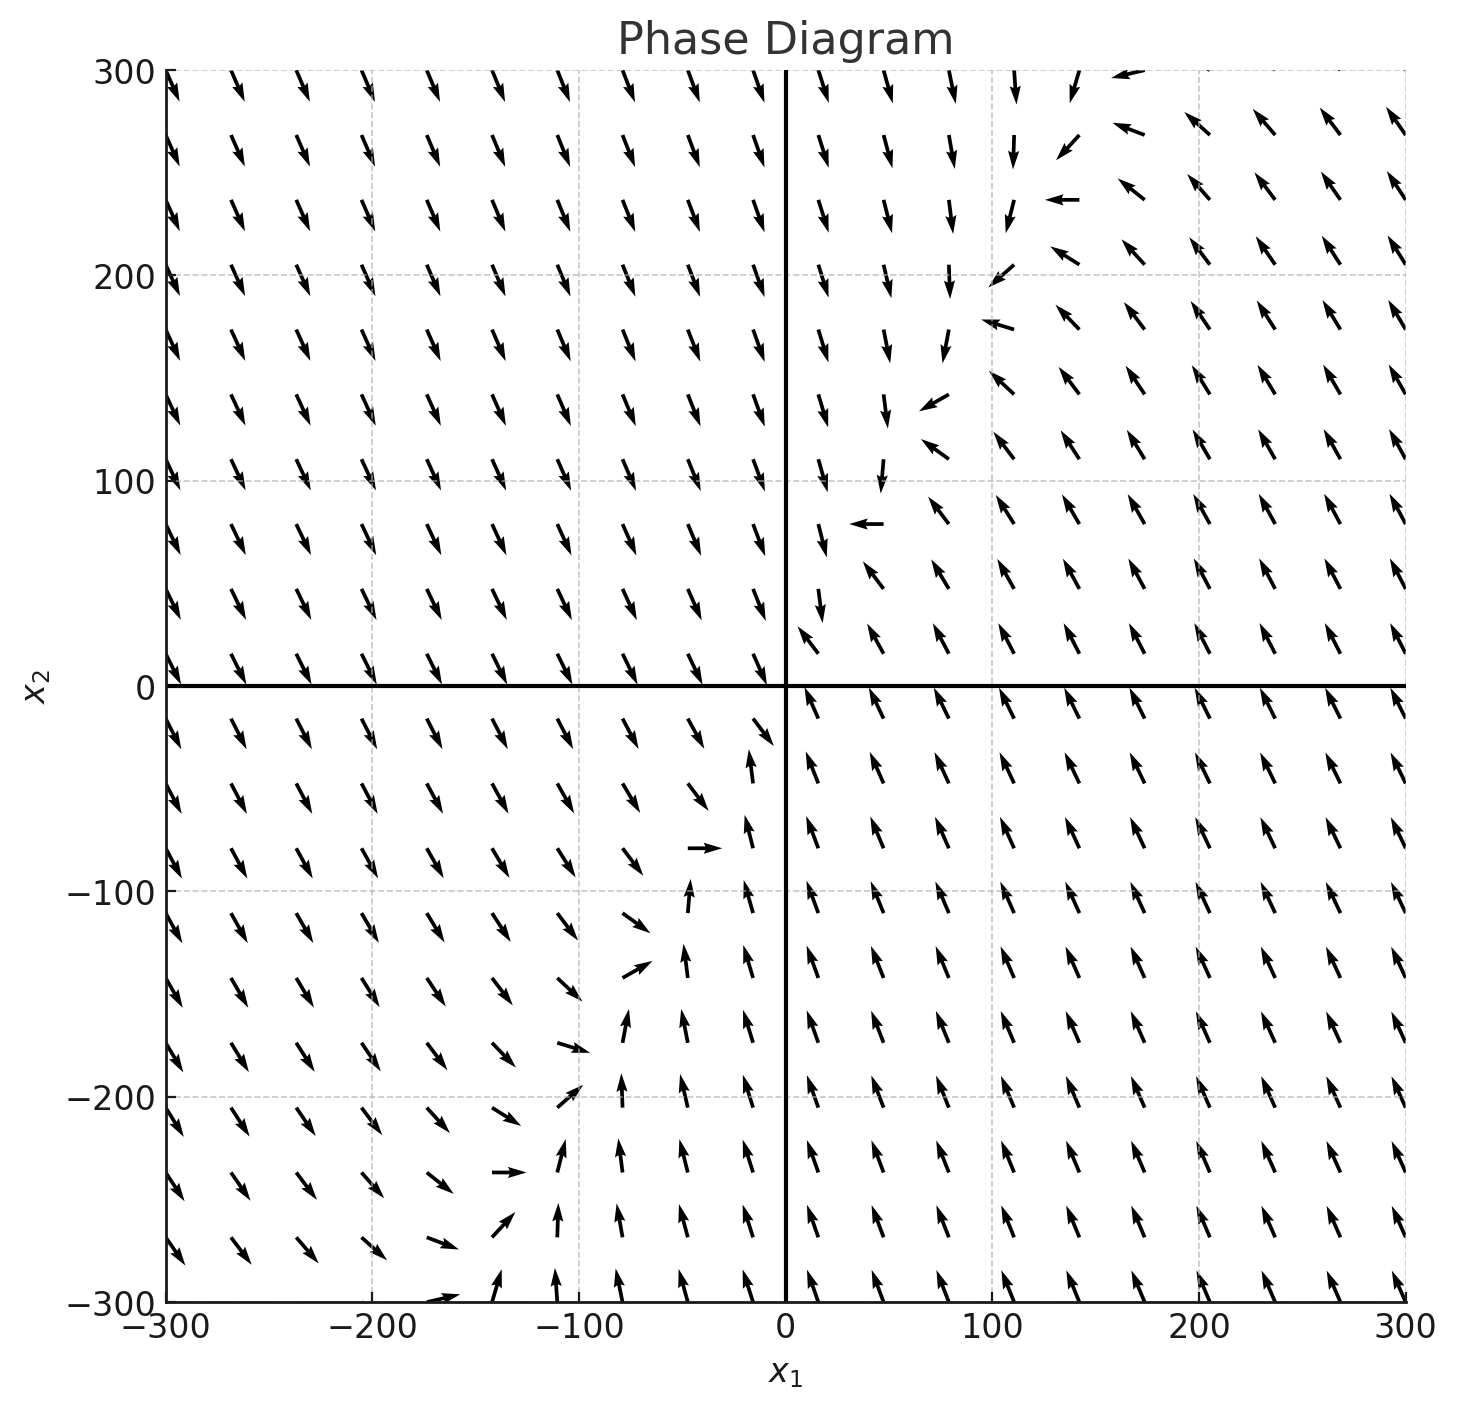
\includegraphics[width=\linewidth]{5_3_16_phase_diagram}


18) The system has two distinct positive real eigenvalues.
This is because it has two lines and is a source.


20) The system has two complex eigenvalues with positive real parts.
This is because it's spiral (complex eigenvalues) and a source (positive real part).


21) The system has one repeated positive real eigenvalue with two linearly
independent eigenvectors. This is because it's a source (positive eigenvalue)
and a proper nodal (repeated non-zero eigenvalue of the same sign).


33) a) Let v be any nonzero vector. We can express v as a linear
combination of $u_1$ and $u_2$ since they are linearly independent
and span the space:
\[v = c_1 v_1 + c_2 v_2\]

where $c_1$ and $c_2$ are scalars.

Since $u_1$ and $u_2$ are eigenvectors are associated with $\lambda$,
we have $A u_1 = \lambda u_1$ and $A u_2 = \lambda u_2$.

We then get:
\[A v = A(c_1 u_1 + c_2 u_2) = c_1 A u_1 + c_2 A u_2 = c_1 \lambda u_1 + c_2 \lambda u_2\]

We can rewrite this as:
\[A v = \lambda (c_1 u_1 + c_2 u_2) = \lambda v\]

This shows that $A v = \lambda v$ for any nonzero vector v. Thus,
every nonzero vector v is an eigenvector of A associated with $\lambda$.

b) Consider $v_1 = \begin{bmatrix}
    1 \\
    0
\end{bmatrix}$ and $v_2 = \begin{bmatrix}
    0 \\
    1
\end{bmatrix}$. These are basis vectors of $\RR^2$.

From part a), we know that $A v = \lambda v$.

For $v_1$,
$A \begin{bmatrix}
    1 \\
    0
\end{bmatrix} = \lambda \begin{bmatrix}
    1 \\
    0
\end{bmatrix}$. This implies that the first column of A
is $\begin{bmatrix}
    \lambda \\
    0
\end{bmatrix}$.

For $v_2$,
$A \begin{bmatrix}
    0 \\
    1
\end{bmatrix} = \lambda \begin{bmatrix}
    0 \\
    1
\end{bmatrix}$. This implies that the second column of A
is $\begin{bmatrix}
    0 \\
    \lambda
\end{bmatrix}$.

Thus, A must be:
\[\begin{bmatrix}
    \lambda & 0 \\
    0 & \lambda
\end{bmatrix}\]

which is exactly the same as equation 22 (a scalar multiple of the
identity matrix).


Section 5.5:

1) Both eigenvalues of the system are -3.
The corresponding eigenvectors are:
$v_1 = \begin{bmatrix}
    0.7071 \\
    -0.7071
\end{bmatrix}$ and $v_2 = \begin{bmatrix}
    -0.7071 \\
    0.7071
\end{bmatrix}$. These eigenvectors are linearly
independent.

For a system of differential equations with a repeated eigenvalue
and linearly independent eigenvectors, the general solution
can be expressed as:
\[x(t) = c_1 e^{\lambda t} v_1 + c_2 e^{\lambda t} v_2\]

Plugging in the values gives:
\[x(t) = c_1 e^{-3t} \begin{bmatrix}
    0.7071 \\
    -0.7071
\end{bmatrix} + c_2 e^{-3t} \begin{bmatrix}
    -0.7071 \\
    0.7071
\end{bmatrix}\]

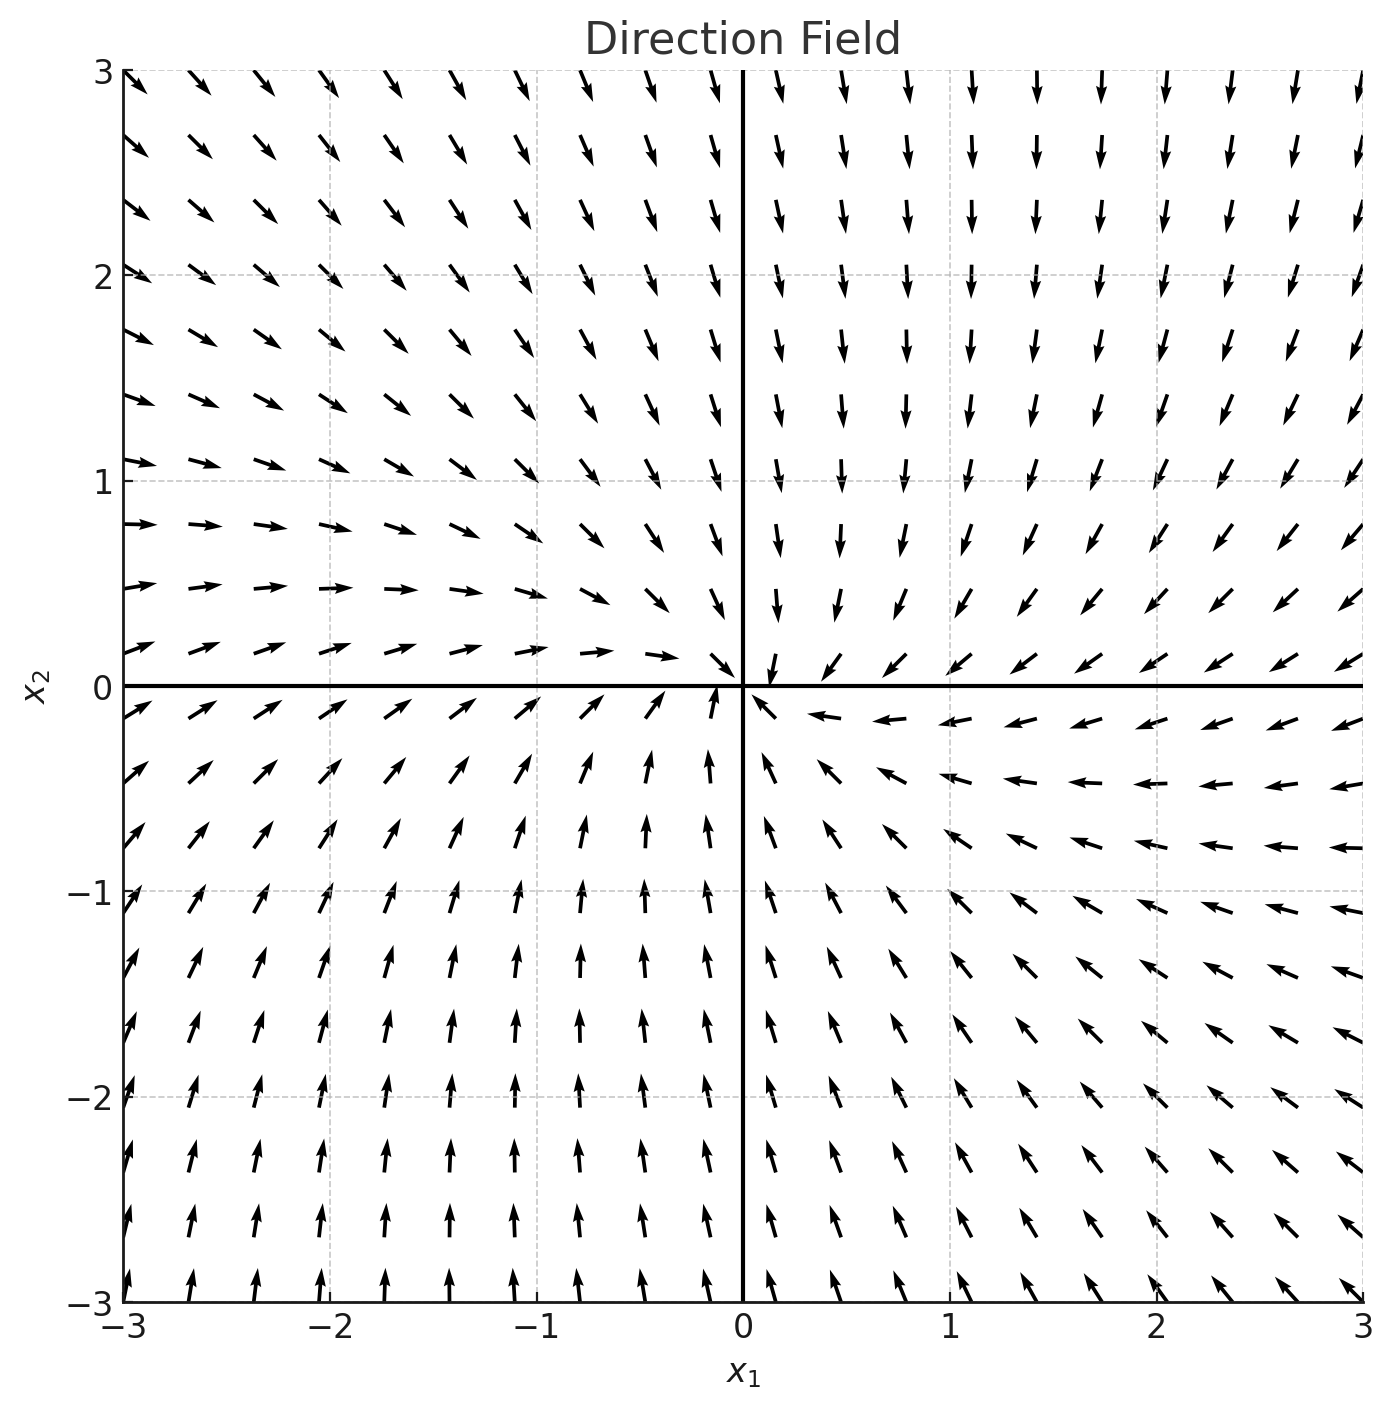
\includegraphics[width=\linewidth]{5_5_1_direction_field}


2) The eigenvalue of the system is 2 (repeated) with only one linearly
independent eigenvector $v = \begin{bmatrix}
    0.7071 \\
    0.7071
\end{bmatrix}$.

In this case, the general solution is given by:
\[x(t) = e^{\lambda t} (c_1 v + c_2 (t v))\]

Plugging in our values gives:
\[x(t) = e^{2t} (c_1 \begin{bmatrix}
    0.7071 \\
    0.7071
\end{bmatrix} + c_2 (t \begin{bmatrix}
    0.7071 \\
    0.7071
\end{bmatrix}))\]

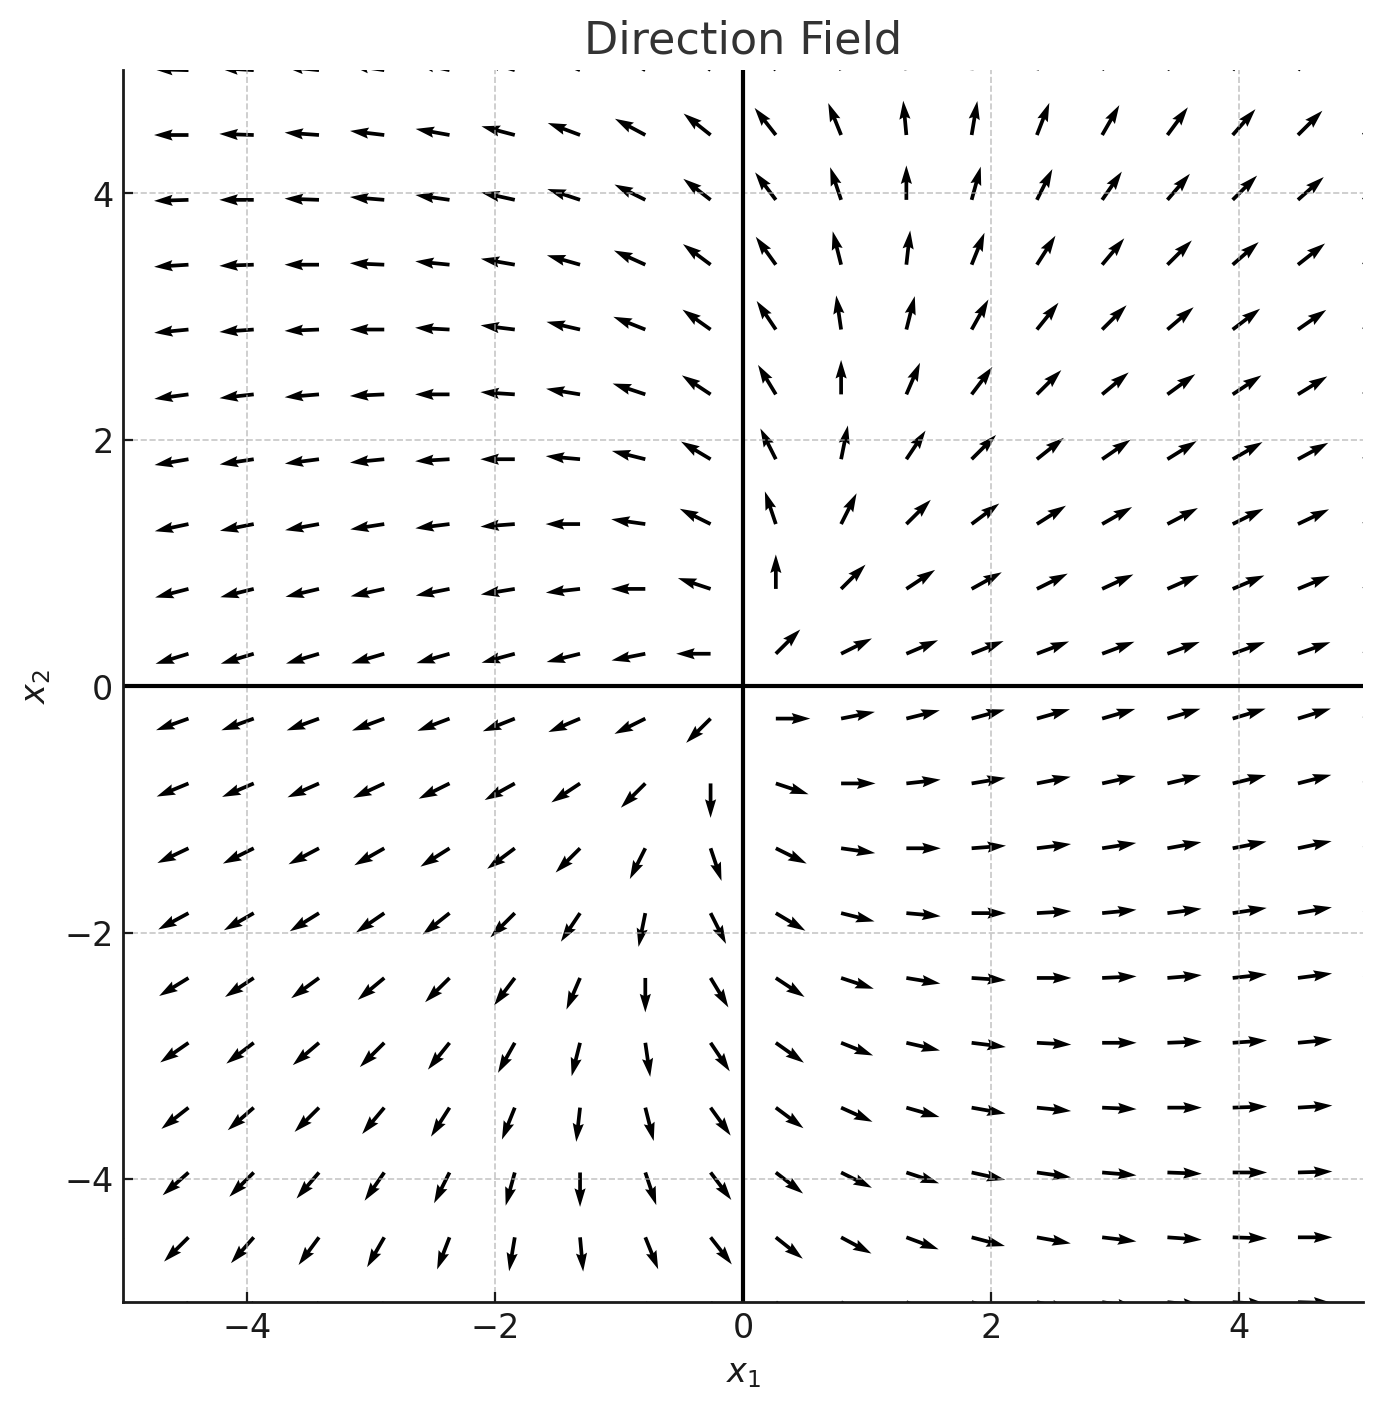
\includegraphics[width=\linewidth]{5_5_2_direction_field}


4) The eigenvalues of the system are both 4. There is only one linearly
independent eigenvector $v = \begin{bmatrix}
    -0.7071 \\
    0.7071
\end{bmatrix}$.

In this case, the general solution is given by:
\[x(t) = e^{\lambda t} (c_1 v + c_2 (t v))\]

Plugging in our values gives:
\[x(t) = e^{4t} (c_1 \begin{bmatrix}
    -0.7071 \\
    0.7071
\end{bmatrix} + c_2 (t \begin{bmatrix}
    -0.7071 \\
    0.7071
\end{bmatrix}))\]

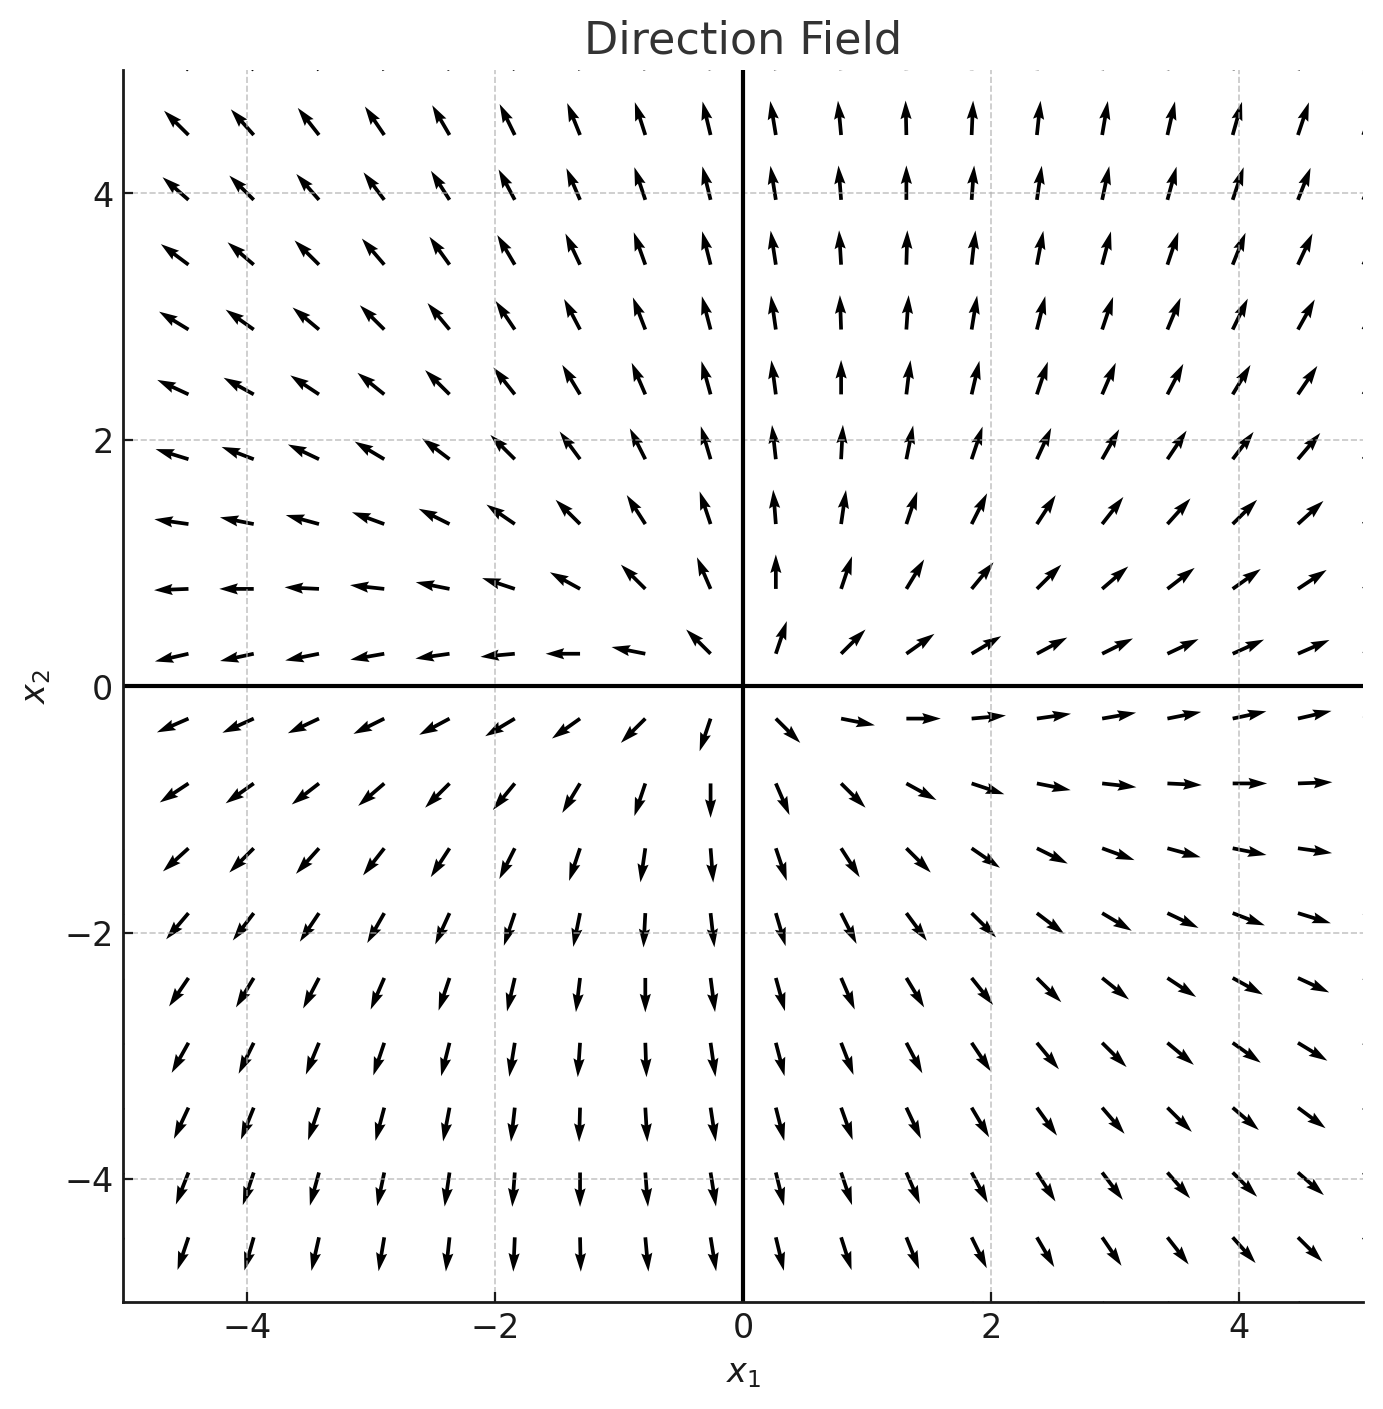
\includegraphics[width=\linewidth]{5_5_4_direction_field}


7) The eigenvalues are 9, 2, andd 2. The corresponding eigenvectors are
$v_1 = \begin{bmatrix}
    0 \\
    1 \\
    0
\end{bmatrix}$, $v_2 = \begin{bmatrix}
    0.7071 \\
    0.7071 \\
    0
\end{bmatrix}$, and $v_3 = \begin{bmatrix}
    0 \\
    -0.7071 \\
    0.7071
\end{bmatrix}$.

The general solution is given by:
\[x(t) = c_1 e^{\lambda_1 t} v_1 + c_2 e^{\lambda_2 t} v_2 + c_3 e^{\lambda_3 t} v_3\]

Plugging in our values we get:
\[x(t) = c_1 e^{9 t} \begin{bmatrix}
    0 \\
    1 \\
    0
\end{bmatrix} + c_2 e^{2 t} \begin{bmatrix}
    0.7071 \\
    0.7071 \\
    0
\end{bmatrix} + c_3 e^{2 t} \begin{bmatrix}
    0 \\
    -0.7071 \\
    0.7071
\end{bmatrix}\]


22) The eigenvalues of the system are all 1 (four eigenvalues with value $\approx 1$).

Note: I used a computer algebra system to calculate the eigenvalues
and eigenvectors for this system (because I don't want to
manually calculate them for a $4 \times 4$ matrix).

The eigenvectors are:
\[v_1 = \begin{bmatrix}
    1 \\
    0 \\
    0 \\
    0
\end{bmatrix}, v_2 = \begin{bmatrix}
    0 \\
    0 \\
    0 \\
    1
\end{bmatrix}\]

I'm not exactly sure how to get the generalized eigenvectors
for the general solution.


28) Here's some code to calculate the general solution
using sympy:

\begin{lstlisting}

import numpy as np
from scipy.linalg import eig
import sympy as sp

# Define the matrix A
A = np.array([[-15, -7, 4], [34, 16, -11], [17, 7, 5]])

# Compute the eigenvectors and eigenvalues
eigenvalues, eigenvectors = eig(A)

# Identify the repeated eigenvalue
repeated_eigenvalue = 2

# Construct the matrix of generalized eigenvectors
# Since there's only one eigenvector,
#  compute two generalized eigenvectors
P = np.column_stack((eigenvectors[:, 0],
        np.linalg.matrix_power(A -
        repeated_eigenvalue*np.eye(3), 1) @ eigenvectors[:, 0],
        np.linalg.matrix_power(A -
        repeated_eigenvalue*np.eye(3), 2) @ eigenvectors[:, 0]))

# Define the symbolic variables for time and constants
t, c1, c2, c3 = sp.symbols('t c1 c2 c3')

# Define the Jordan matrix
J = sp.Matrix(np.diag([repeated_eigenvalue]*3))
J[0, 1] = J[1, 2] = 1  # Filling the superdiagonal with 1's

# General solution
# x(t) = P * exp(J*t) * c, where c is the vector of constants
c = sp.Matrix([c1, c2, c3])
x_t = sp.Matrix(P) * sp.exp(J * t) * c

print(x_t)

\end{lstlisting}


34) We need to show that $(A - \lambda I_n) v_2 = v_1$
and $(A - \lambda I_n) v_1 = 0$.

If we actually do the calculations (omited for brevity
since it's just some matrix arithmetic),
then we will get what we need to show.

Therefore, $v_1$ and $v_2$ do form a length 2 chain associated with
the eigenvalue $\lambda = 2 + 3i$.

The four independent real-valued solutions are:

1. \[\begin{bmatrix}
    e^{2t} \sin(3t) \\
    (-3 \sin(3t) + 3 \cos(3t)) e^{2t} \\
    0 \\
    -e^{2t} \cos(3t)
\end{bmatrix}\]

2. \[\begin{bmatrix}
    -e^{2t} \sin(3t) \\
    (3 \sin(3t) + 3 \cos(3t)) e^{2t} \\
    0 \\
    -e^{2t} \cos(3t)
\end{bmatrix}\]

3. \[\begin{bmatrix}
    3e^{2t} \cos(3t) \\
    (-9 \sin(3t) - 10 \cos(3t)) e^{2t} \\
    e^{2t} \sin(3t) \\
    0
\end{bmatrix}\]

4. \[\begin{bmatrix}
    3e^{2t} \cos(3t) \\
    (9 \sin(3t) - 10 \cos(3t)) e^{2t} \\
    -e^{2t} \sin(3t) \\
    0
\end{bmatrix}\]


Textbook Section 5.6:

1) The fundamental matrix is:
\[\phi(t) = \begin{bmatrix}
    0.5e^t + 0.5e^{3t} & -0.5e^t + 0.5e^{3t} \\
    -0.5e^t + 0.5e^{3t} & 0.5e^t + 0.5e^{3t}
\end{bmatrix}\]

Applying equation 8 for $x(0) = \begin{bmatrix}
    3 \\
    -2
\end{bmatrix}$ yields the solution:
\[x(t) = \begin{bmatrix}
    2.5e^t + 0.5e^{3t} \\
    -2.5e^t + 0.5^{3t}
\end{bmatrix}\]


22) Let's first try to prove that its nilpotent by computing successive
powers of A.

If we compute $A^2$, we end up with $A^2 = \begin{bmatrix}
    0 & 0 \\
    0 & 0
\end{bmatrix}$, which is the null matrix, therefore
A is nilpotent and powers $\geq 2$ give the zero $2 \times 2$ matrix.

That means that $e^{At}$ is given by:
\[e^{At} = I_n + A t\]

Plugging in A, we get that:
\[e^{At} = \begin{bmatrix}
    6t + 1 & 4t \\
    -9t & 1 - 6t
\end{bmatrix}\]


28) First, notice that $A = D + N$
where $D = 5 I_n$ and $N = \begin{bmatrix}
    0 & 0 & 0 \\
    10 & 0 & 0 \\
    20 & 30 & 0
\end{bmatrix}$.
Note that $e^{At} = e^{(D + N)t} = e^{Dt} e^{Nt}$.
Finally, $x(t) = e^{At} x(0)$.

\[e^{At} = \begin{bmatrix}
    e^{5t} & 0 & 0 \\
    10te^{5t} & e^{5t} & 0 \\
    (150t^2 + 20t)e^{5t} & 30te^{5t} & e^{5t}
\end{bmatrix}\]

That means that $x(t) = \begin{bmatrix}
    40e^{5t} \\
    400te^{5t} + 50e^{5t} \\
    1500te^{5t} + 40(150t^2 + 20t)e^{5t} + 60e^{5t}
\end{bmatrix}$


\end{document}
